\subsection{Data Description}\label{subsec:climate_description}

Climate variables were extracted from the \textit{WorldClim v2.1} monthly weather dataset at a spatial resolution of 5 arc-minutes (approximately 10 km). The study area covers Algeria and Tunisia, and the temporal scope spans the period 2020–2024. Three monthly climate variables were considered:
\begin{itemize}
    \item Total precipitation (\texttt{prec\_mm}, in millimeters),
    \item Maximum temperature (\texttt{tmax\_c}, in degrees Celsius),
    \item Minimum temperature (\texttt{tmin\_c}, in degrees Celsius).
\end{itemize}

Each variable was sampled on a common spatial grid using centroid-based extraction, yielding identical spatial coverage and temporal resolution. The resulting datasets have identical shapes:
\begin{itemize}
    \item Precipitation: $(1\,399\,320,\ 4)$,
    \item Maximum temperature: $(1\,399\,320,\ 4)$,
    \item Minimum temperature: $(1\,399\,320,\ 4)$.
\end{itemize}

Each dataset occupies approximately 42.7 MB in memory. All temperature values are expressed in degrees Celsius, ensuring physical interpretability and consistency across analyses.

\subsection{Data Visualization}\label{subsec:climate_visualization}

\subsubsection{Distribution Analysis}

Figure~\ref{fig:climate_histograms} presents the empirical distributions of precipitation, maximum temperature, and minimum temperature. Precipitation exhibits a highly right-skewed distribution, with a large concentration of low values and a long tail corresponding to intense rainfall events. This behavior is typical of semi-arid and Mediterranean climates, where dry conditions dominate most months.

Maximum and minimum temperatures display broader, multi-modal distributions reflecting strong seasonal variability. The separation between cold and warm regimes is clearly visible, with minimum temperatures spanning from sub-zero values to above $30^\circ$C, and maximum temperatures reaching nearly $50^\circ$C in extreme summer conditions.

\begin{figure}[H]
    \centering
    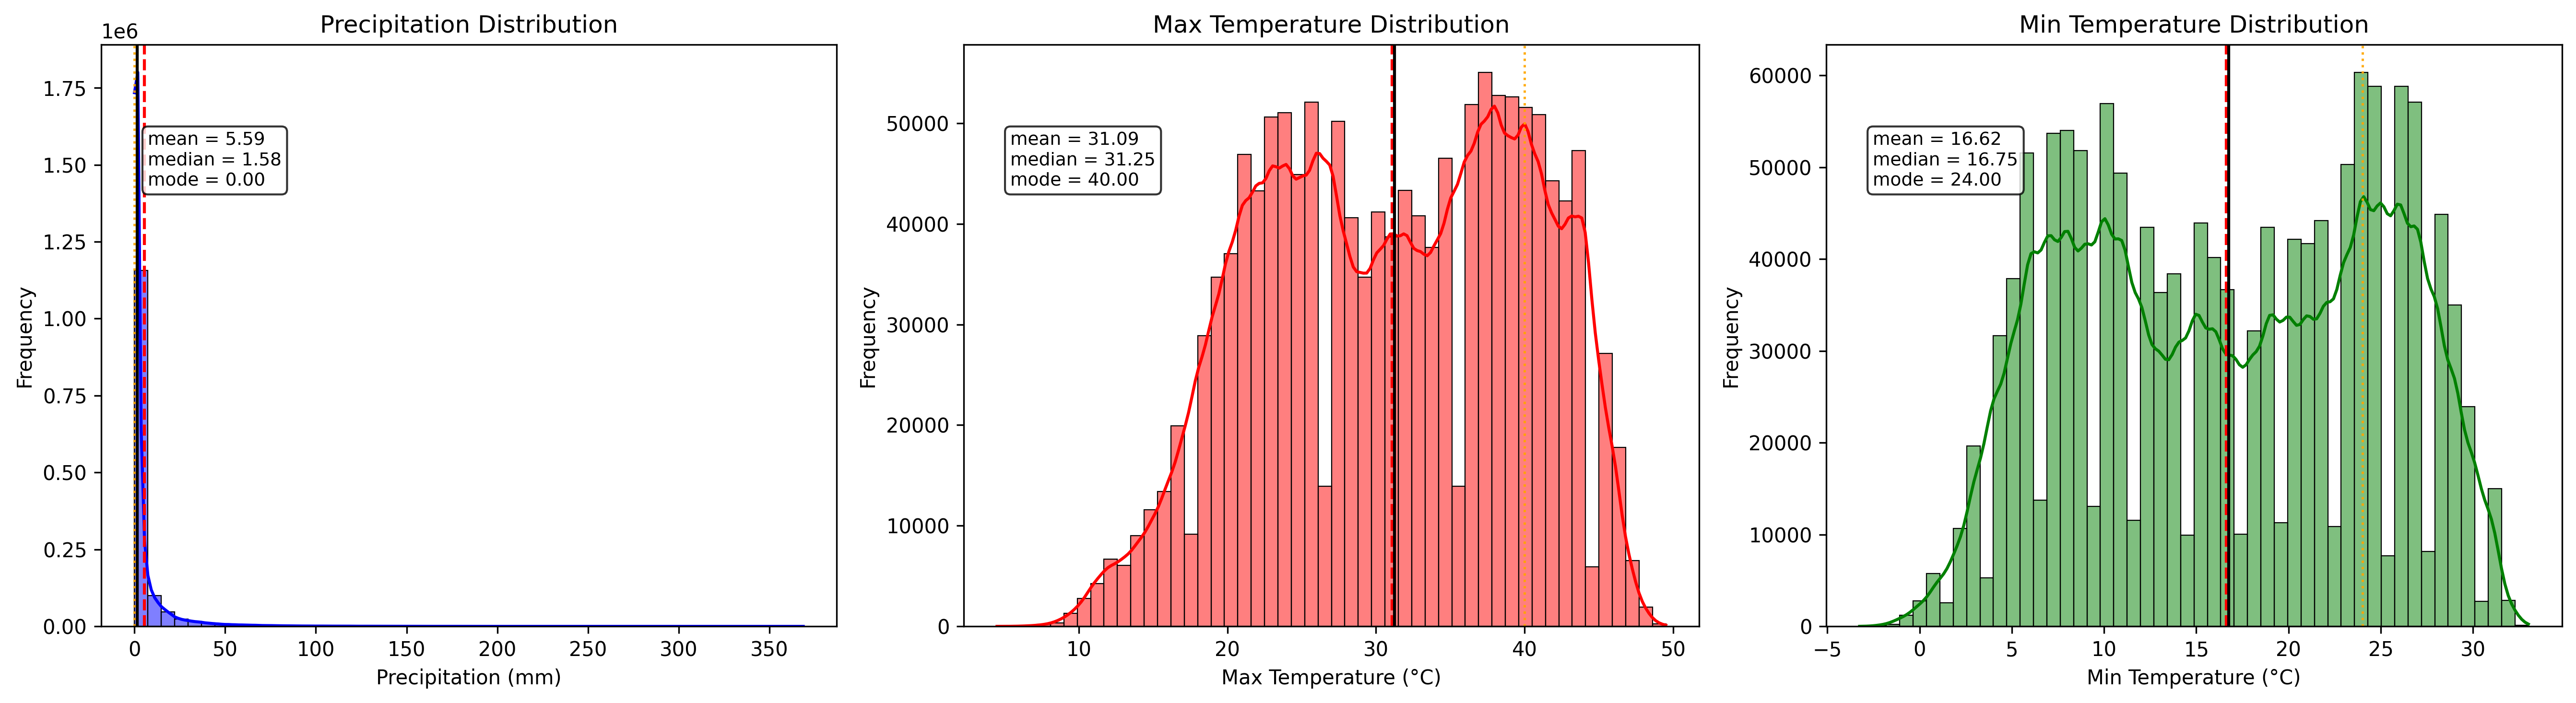
\includegraphics[width=0.95\linewidth]{images/Climate/climate_histograms_raw.png}
    \caption{Histograms of raw climate variables: precipitation, maximum temperature, and minimum temperature.}
    \label{fig:climate_histograms}
\end{figure}

Kernel Density Estimation (KDE) plots after imputation (Figure~\ref{fig:climate_kde}) confirm these observations. Precipitation remains strongly right-skewed, while temperature variables show smoother, multi-peaked density functions corresponding to seasonal cycles.

\begin{figure}[H]
    \centering
    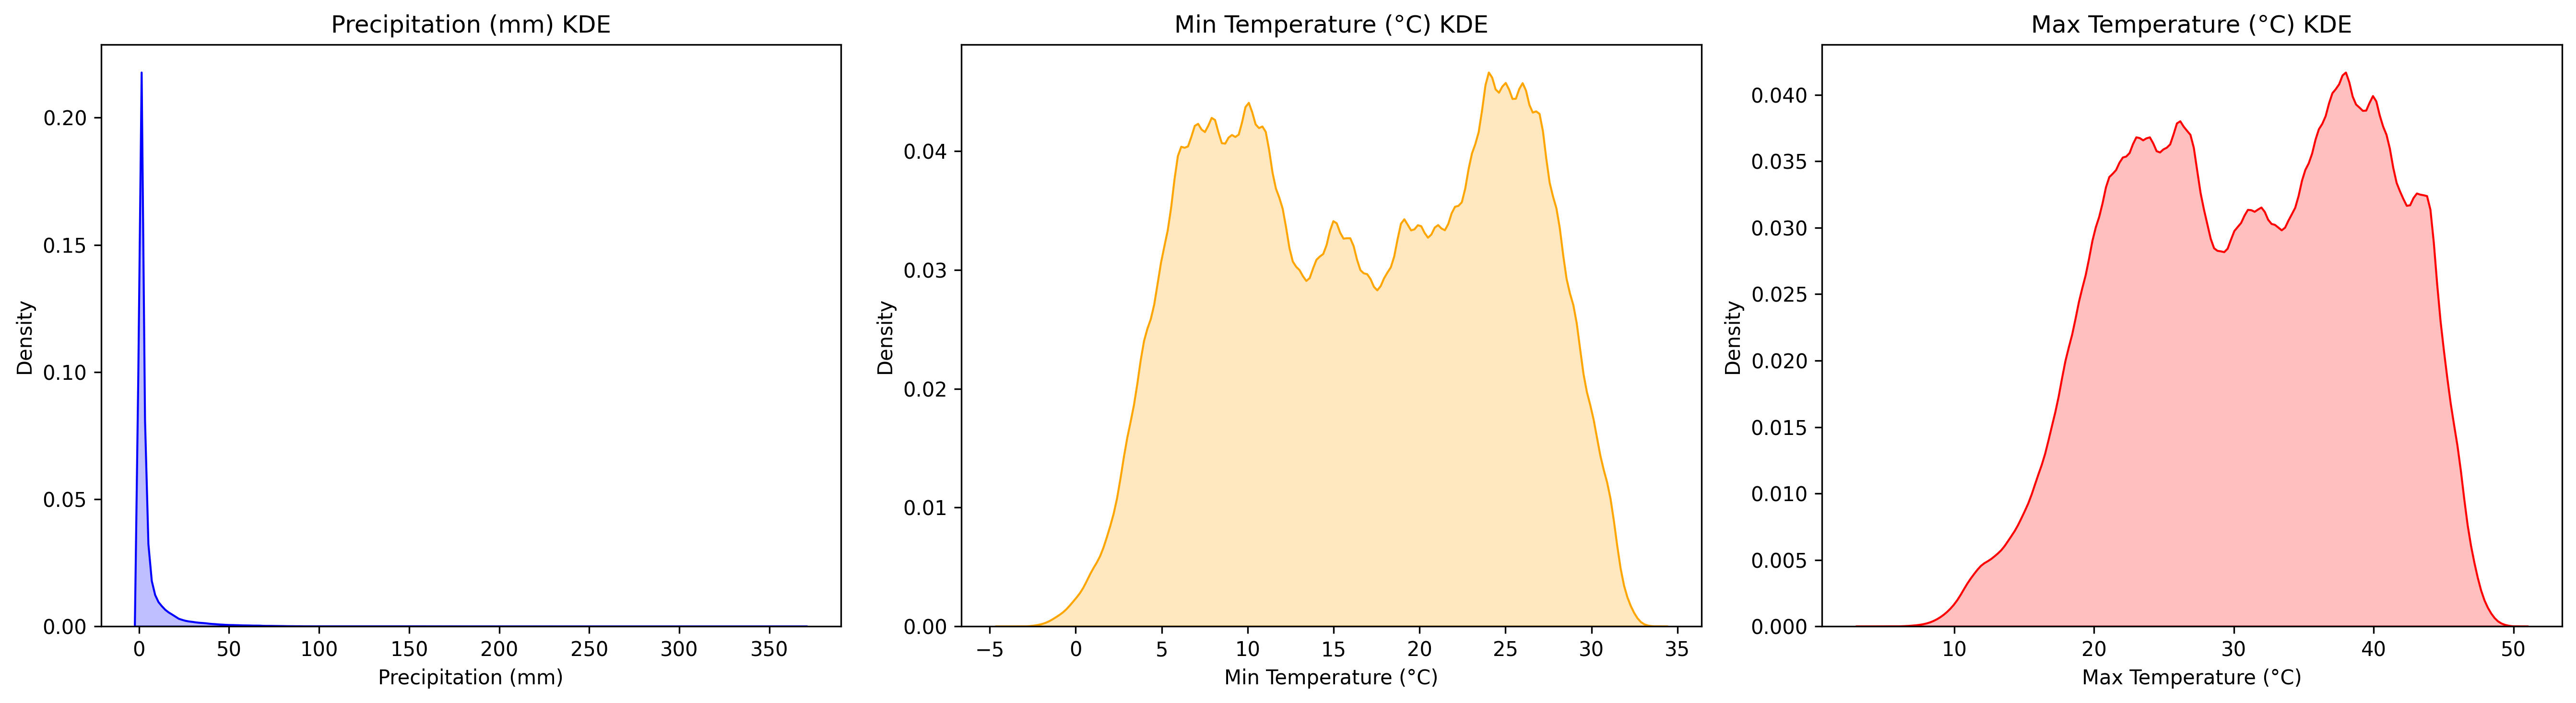
\includegraphics[width=0.95\linewidth]{images/Climate/climate_kde_imputed.png}
    \caption{Kernel density estimates of imputed climate variables.}
    \label{fig:climate_kde}
\end{figure}

\subsubsection{Normality Assessment}

Q--Q plots (Figure~\ref{fig:climate_qq}) indicate strong deviations from normality for precipitation, particularly in the upper quantiles, confirming the presence of heavy tails. Temperature variables exhibit more linear behavior in central quantiles but still deviate at the extremes, reflecting bounded physical processes and seasonal effects. These results indicate that no climate variable follows a Gaussian distribution, justifying the use of normalization or robust scaling rather than assumptions of normality.

\begin{figure}[H]
    \centering
    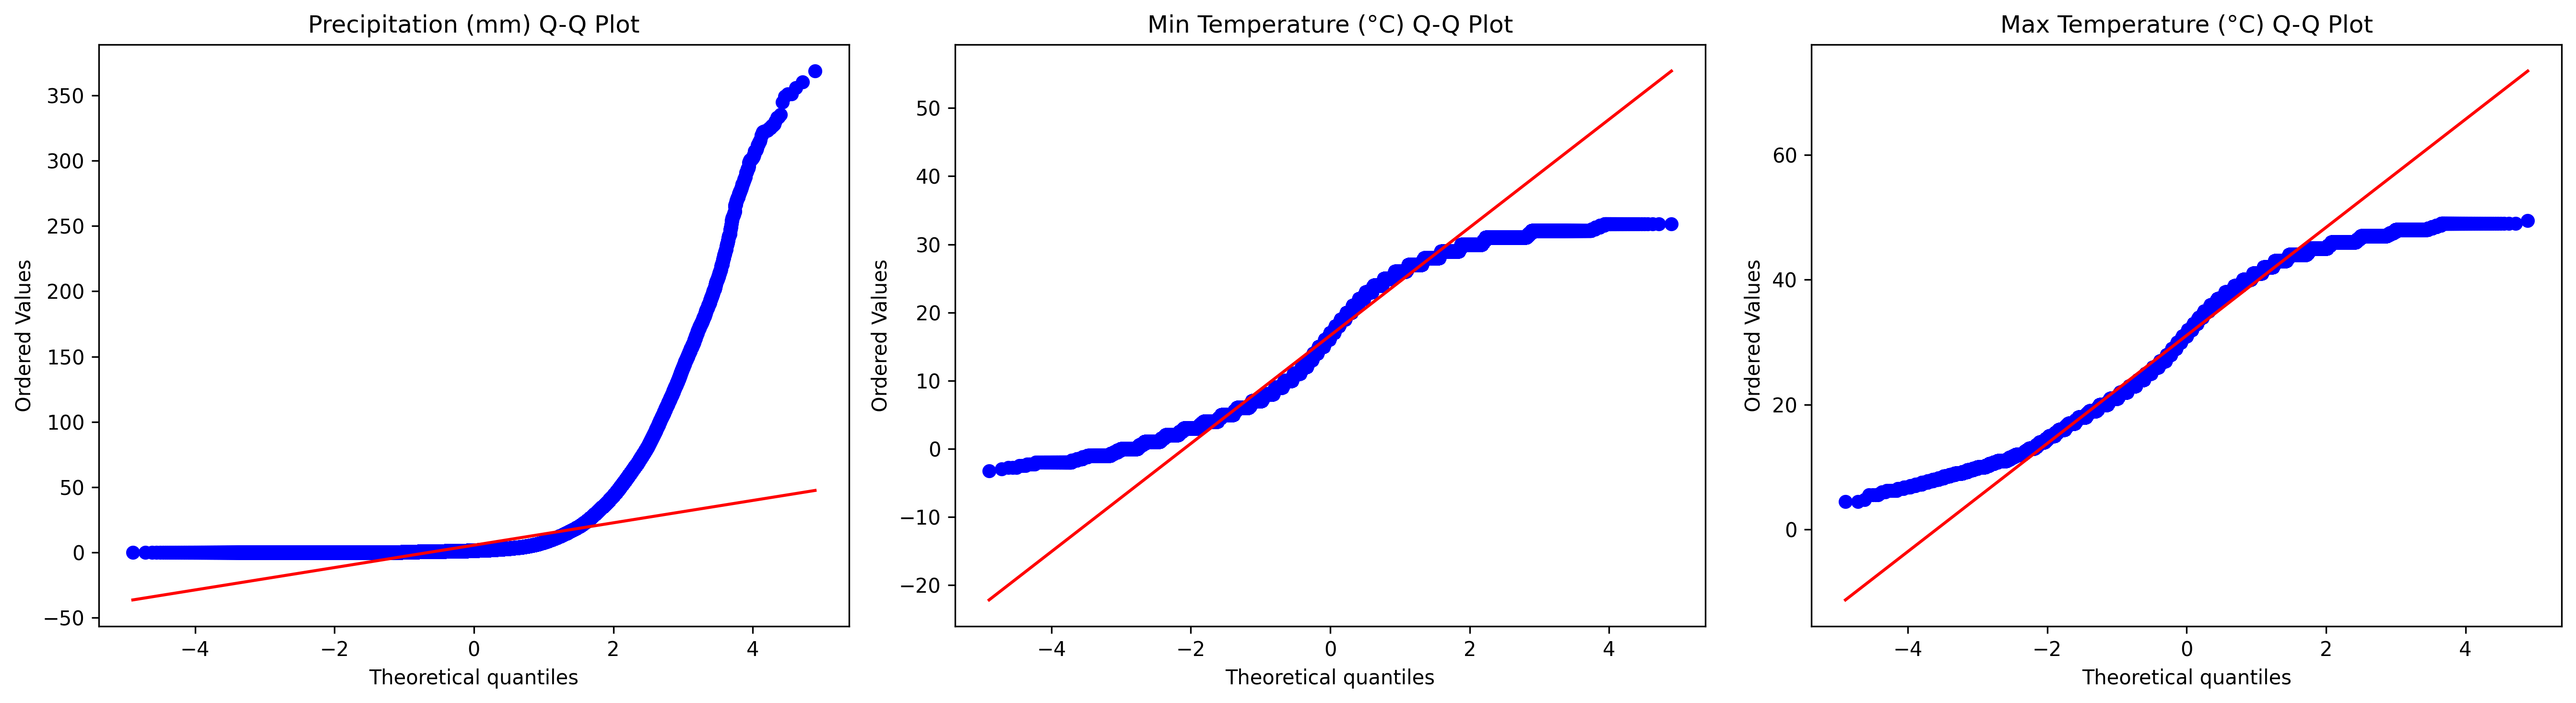
\includegraphics[width=0.95\linewidth]{images/Climate/climate_qq_plots_imputed.png}
    \caption{Q--Q plots for precipitation, minimum temperature, and maximum temperature after imputation.}
    \label{fig:climate_qq}
\end{figure}

\subsubsection{Spatial Patterns}

The figure in the Annex~\ref{annexe:climate-viz-summary} illustrates spatial heatmaps of mean climate conditions over the 2020–2024 period. Precipitation shows a strong north–south gradient, with wetter conditions in northern coastal and mountainous regions and extremely dry conditions in the Saharan south. Temperature maps display the inverse pattern: higher maximum and minimum temperatures dominate southern regions, while cooler conditions prevail at higher latitudes and elevations.

Monthly snapshot maps further highlight seasonal contrasts, particularly for January, where temperature gradients are most pronounced.
